\setlength{\parskip}{\baselineskip}%
\setlength{\parindent}{0pt}%

In the winter of 1868/9, Swiss physician and biologist, Johannes Friedrich Miescher isolated an unknown substance from the nuclei of cells\cite{dahm2008discovering}. This substance was unlike anything he had observed before; it was resistant to protease, lacked sulphur and contained large amounts of phosphorous. He recognised that he had isolated a novel substance and since it was isolated from the nucleus, he named it nuclein. Today, we know of this substance as deoxyribonucleic acid (DNA), the molecule of heredity.

Although Miescher speculated that nuclein may have had a role in heredity, he later rejected the idea. It wasn't until 1944, when Oswald Avery, Colin MacLeod, and Maclyn McCarty characterised the transforming factor in Griffith's Experiment\cite{griffith1928significance} as DNA, that it was hypothesised that DNA was the genetic material\cite{avery1944studies}. In order to identify DNA as the transforming factor, they used an enzyme that only degraded DNA (deoxyribonucleodepolymerase) and showed that it was able to eliminate the transforming power. It was later confirmed in 1952 by Alfred Hershey and Martha Chase that DNA is indeed the genetic material by performing a series of experiments in viruses that infected bacteria (bacteriophages)\cite{hershey1952independent}. They demonstrated that when the bacteriophages infected bacteria, only their DNA would enter into the cytoplasm of the bacteria, proving that DNA was indeed the genetic material.

Fast forward to the 21st century and not only have we sequenced the entire collection of DNA, the genome, of our very own species \cite{venter2001sequence, lander2001initial}, we have the capacity to sequence an entire human genome in a matter of days by using high-throughput sequencers. We have also just recently reached the \$1,000 genome era, whereby we can sequence the entire genome of an individual for around \$1,000 US dollars (USD). In contrast, the Human Genome Project, which gave us the first glimpse of the human genome costed approximately 2.7 billion fiscal year 1991 US dollars\cite{nhgri2010cost}. In just ~60 years, we have gone from establishing that DNA is the molecule of heredity to being able to sequence a human genome in a few days for around 1,000 USD.

However, high-throughput sequencing is not limited to genome sequencing. The discovery of reverse transcriptase\cite{pmid4316300, pmid4316301} allowed the generation of complementary DNA (cDNA) from an ribonucleic acid (RNA) template; thus we are able to sequence the entire collection of RNA, known as the transcriptome, from biological samples. Various molecular biology techniques when coupled with sequencing allowed the capture of DNA-protein interactions, DNA methylation patterns, histone modifications, and a growing number of applications\cite{applicationsofsequencing}. While the genome is assumed to be more or less identical in the estimated 37 trillion cells in the human body\cite{pmid23829164}, the transcriptome is much more variable. It is the differential use of the genome that is thought to give rise to over 400 different cell types\cite{pmid16790079} that make up a human.

It is the comparison of different transcriptomes, captured from different cell types or samples treated under different treatment regimes, that allows the characterisation of RNA that are implicated in various functions. This thesis is about the use of high-throughput sequencing in a collection of transcriptomic studies investigating several biological problems. The first paper examined a particular biases that arose in the use high-throughput transcriptome profiling and demonstrated how such biases can be avoided\cite{Tang01022013}. The second paper was a study investigating the role of small RNAs in the DNA damage repair process, which used small RNA sequencing to identify a new class of small RNA\cite{francia2012site}. The third paper was a study on human induced pluripotent stem cells (iPSCs) and the use of transcriptome profiling to explore the role of a chemokine in iPSCs. The fourth paper focused on a particular class of DNA known as repetitive elements and investigated the RNA expression of such elements. The fifth paper was a study involving the profiling of RNA in whole blood and how such an approach maybe useful for finding biomarkers. The sixth and last paper investigates a particular class of small RNA known as piwi-interacting RNA (piRNA) and proposes a role of piRNAs in Rett syndrome.

\section{What are genes?}

The classical definition of a gene dates back to Gregor Mendel when he noticed that discrete traits could be inherited from the parents to the offspring in his plant breeding experiments. While the mechanism of inheritance wasn't clear, these heritable traits were termed a gene. The definition of a gene has evolved as our knowledge of genetics evolved\cite{pmid17567988}. To understand the relationship between DNA and genes requires a molecular understanding of DNA. After Johannes Friedrich Miescher discovered nuclein, Albrecht Kossel in 1881 determined that nuclein is composed of five bases: adenine, cytosine, guanine, thymine, and uracil, which are commonly abbreviated as A, C, G, T, and U. Later in 1889, Richard Altmann discovered that nuclein is acidic and renames it as nucleic acid and in 1909 Phoebus Levene discovered that DNA consists of three basic components: an acid, an organic base, and a sugar. Today we know that these three components are a base, a phosphate, and a pentose. There are two types of pentoses: ribose and 2-deoxyribose; compounds that consist of a base and a pentose are called nucleosides. In nucleosides, if phosphates are linked to the hydroxyl group of their sugar then they become nucleotides or nucleic acids; this sugar-phosphate backbone forms the structural framework of nucleic acids. Nucleic acids with a ribose sugar are known as ribonucleic acid (RNA) and those with a 2-deoxyribose sugar are known as deoxyribonucleic acid (DNA).

Chargaff's rules by Erwin Chargaff

When the three-dimensional structure of DNA was deduced\cite{WATSON_1953} it became apparent how DNA could function as the molecule of heredity. 

In their paper they famously said:

\epigraph{``It has not escaped our attention that the specific pairing we have postulated immediately suggests a possible copying mechanism for the genetic material."}{--- \textup{Watson and Crick}}

The nucleotides are the molecular building-blocks of DNA and RNA.

form what is called the genetic code\cite{pmid5330357}, which defines how information is encoded in the genetic material. 

In eukaryotes, three nucleotides define a codon, which is translated into a corresponding amino acid. There are only 20 standard amino acids, despite having 64 codon permutations; this is because the genetic code is degenerate, meaning that different codons code for the same amino acid. Thus some single nucleotide polymorphisms (SNPs) may not change the amino acid; these mutations are known as synonymous mutations. DNA mutations that cause a different amino acid to be coded are known as non-synonymous mutations. 

The relationship between genes and proteins


\section{The human genome}

\begin{itemize}

   \item The genome is all the chromosomes in a cell
   \item A chromosome is a long DNA molecule and some associated proteins
   \item Divided into genes, which is a section of DNA that is used in producing a particular protein
   \item In each gene, the chemicals are arranged in specific ways to facilitate the production of specific proteins
   \item Every time a protein in needed, the appropriate chemical code is read off the gene; this gives the pattern of chemical elements that will make that protein what it is
   
\end{itemize}

Genes to proteins to pathways to sub-cellular mechanisms to cells to tissues to organs to organism

Living cell where molecules, such as proteins, interact and change.

Most cells in the human body are diploid, containing 23 pairs of chromosomes. The haploid human genome contains ~3\e{9} base pairs of DNA; this makes a total of 6 billion base pairs of DNA per cell. Each base pair of DNA is ~0.34 nanometers long or 3.4\e{-10} meters\cite{pmid7354864}.

Therefore each diploid cell contains around 2 meters of DNA (3.4\e{-10} * 3\e{9}). From BioNumbers\cite{pmid23829164}, it is estimated that the total cell number in body 3.7\e{13} or 37 trillion cells; so we have around 74 trillion meters of DNA in us.

Certain proteins, called histones, help compact the vast amounts of DNA inside of us (specifically, inside the eukaryotic nucleus). The histones are a family of small, positively charged proteins that provide the energy, in the form of electrostatic interactions, to fold negatively charged DNA (due to the phosphate groups in its phosphate-sugar backbone). The resulting DNA-protein complex is called chromatin.

The packaging of DNA into nucleosomes shortens the fiber length about sevenfold. So a piece of DNA that's 1 meter long, will become ~14 centimeters long (100/7) after wrapping around histones. However despite this, chromatin is still too long to fit inside the nucleus, which is ~10 to 20 microns in diameter. Chromatin is further coiled into a thicker fiber, called the 30nm fiber, because it is roughly 30 nanometers in diameter. Histone H1 is very important in stabilising higher-order chromatin, and 30nm fibers form most readily when H1 is present.

Processes such as transcription and replication require the two strands of DNA to come apart temporarily, thus allowing polymerases access to the DNA template. However, the presence of nucleosomes and the folding of chromatin into 30-nanometer fibers pose barriers to the enzymes that unwind and copy DNA. It is therefore important for cells to have means of opening up chromatin fibers and/or removing histones transiently to permit transcription and replication to proceed. Generally speaking, there are two major mechanisms by which chromatin is made more accessible:

\begin{enumerate}
   \item Histones can be enzymatically modified by the addition of acetyl, methyl, or phosphate groups.
   \item Histones can be displaced by chromatin remodelling complexes, thereby exposing underlying DNA sequences to polymerases and other enzymes.
\end{enumerate}

It is important to remember that these processes are reversible, so modified or remodelled chromatin can be returned to its compact state after transcription and/or replication are complete.

\subsection{DNA sequencing}

\subsection{Sanger / Maxam-Gilbert sequencing}

\subsection{Sequencing by synthesis}

\section{Applications of sequencing}

The age of high throughput sequencing and the application of this technology to studying the transcriptome (also epigenome and interactome)

\subsection{Transcriptomics}

The transcriptome is the collection of RNA molecules derived from the genome at a particular time and location. The diversity of cells is determined by the expression patterns of genes and transcription factors (TFs).

\subsection{Transcription}

The genome is a store of biological information but requires the coordinated activity of enzymes and proteins to bring about transcription. Chromatin structure and nucleosome positioning are altered in order for the transcriptional machinery to access parts of the genome for transcription. The pre-initiation complex that contains RNA polymerase II and general transcription factors forms near the core promoter region around the transcription start site and primes RNA polymerase II for transcription. Processing of precursor RNA include the addition of a cap and poly-A tail, splicing, and RNA editing. Removal of the cap is considered to the first step towards mRNA degradation. The capping procedure is thought to occur only in the nucleus, however a cytoplasmic form of a capping enzyme has been identified; the role of cytoplasmic re-capping.

\subsection{RNA polymerase}

\subsection{Reverse transcription}

\begin{itemize}

   \item Studies on the yeast transcriptome using DNA microarrays showed that although mRNAs are being degraded and re-synthesised all the time, the composition of the yeast transcriptome undergoes very little change if the environment remains constant
   \item However on switching from aerobic to anaerobic respiration, the levels of over 700 mRNAs increase by a factor of two or higher, and another 1,000 mRNAs decline to less than half their original amount
   \item Studying the transcriptome of acute lymphoblastic leukemia cells with respect to acute myeloid leukemia cells revealed differences that made it possible to distinguish the two types of leukemia
   \item Collection of full length cDNAs by the FANTOM consortium revealed many transcripts of unknown function (TUFs)
   \item The technologies that allowed full length cDNA sequencing
   \item Cap Analysis Gene Expression (CAGE) for genome-wide identification of transcription start sites
   \item Biotinylation of diol groups of RNA (High Efficiency Selection of Full-length cDNA by Improved Biotinylated Cap Trapper)
   \item PacBio sequencing has read lengths greater than 10kb and can be used for full length cDNA sequencing

\end{itemize}

\section{The repetitive genome}

Since the release of the draft human genome sequence\cite{venter2001sequence, lander2001initial}, it was established that only a small fraction of the genome is made up of protein-coding sequences and the majority of the genome was made up with repetitive elements. As the human genome contains the entire instruction set that is necessary for the development of a human, the decoding of the genome was thought to provide answers to many outstanding biological questions. However, there are several paradoxes that are still currently unresolved:

\begin{enumerate}
   \item K-value paradox: complexity does not correlate with the number of chromosomes
   \item C-value paradox: complexity does not correlate with genome size
   \item N-value paradox: complexity does not correlate with the number of protein coding genes
\end{enumerate}

If we measure organismal complexity in terms of mental cognition, we observe that complexity is not correlated to the number of chromosomes, the size of genomes, and the number of protein coding genes. Humans have 46 chromosomes and some species of butterflies have over hundreds of chromosomes, such as \textit{Polyommatus atlantica}. In terms of genome size, the species \textit{Polychaos dubium}, a freshwater amoeboid, has one of the largest genomes known with ~670 gb of DNA sequence; humans on the other hand have a genome size of ~3 gb. And lastly humans have roughly the same number of protein-coding genes as \textit{Caenorhabditis elegans}, ~20,000 versus ~21,000, respectively. However, the \textit{C. elegans} genome is ~100 mb\cite{celegans1998sequencing}, which is ~30 times smaller than the human genome, despite having a similar number of genes. One of the discrepancies between genome sizes despite having a similar number of genes is due to repetitive elements, which makes up roughly 50\% of the human genome. Among 66 vertebrate genomes, the percentage coverage of repetitive elements in the human genome is quite high (Figure ~\ref{fig:repeat_coverage_vertebrate_genome}).

\begin{figure}[h]
   \centering
   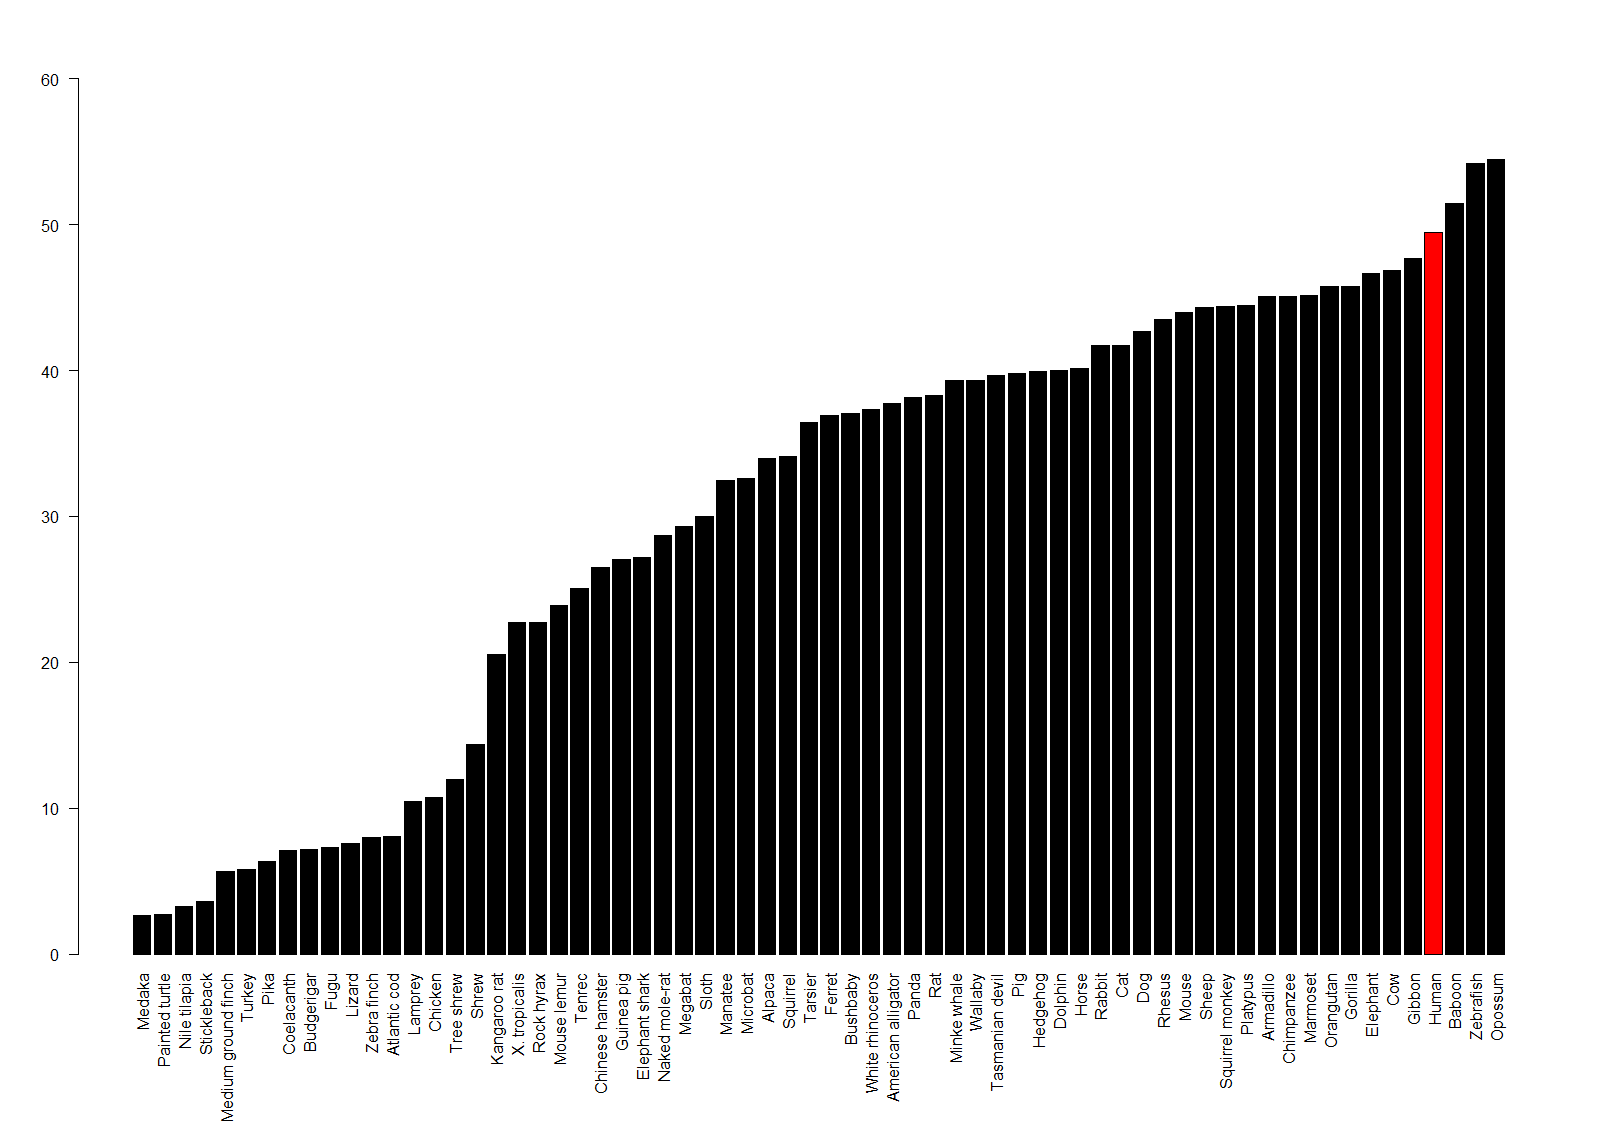
\includegraphics[width=\textwidth,natwidth=1600,natheight=1148]{repeat_coverage_vertebrate_genome.png}
   \caption[Coverage of repetitive elements in vertebrate genomes]{The total coverage of repetitive element in 66 vertebrate genomes as annotated by RepeatMasker in the respective genomes\cite{tang2014repcoverage}.}
   \label{fig:repeat_coverage_vertebrate_genome}
\end{figure}

However, the larger vertebrate genomes do not always contain the highest percentage of repetitive elements (Figure ~\ref{fig:genome_size}). At least in humans, transposons make up the majority of the repetitive elements that make up the human genome. In particular class I transposons (retrotransposons), which are able to transcribed and inserted into the genome, make up a large portion of the human genome. W.Ford Doolittle and Carmen Sapienza wrote in 1980\cite{doolittle1980selfish}: "When a given DNA, or class of DNAs, of unproven phenotypic function can be shown to have evolved a strategy (such as transposition) which ensures its genomic survival, then no other explanation for its existence is necessary" and Leslie Orgel and Francis Crick, wrote that junk DNA has little specificity and conveys little or no selective advantage to the organism\cite{orgel1980selfish}.

The origin of the term "junk DNA" is usually attributed to Susumu Ohno, who used it to describe pseudogenes, which are gene copies that have no known biological function. In its modern day usage, "junk DNA" is used to describe DNA sequence that goes not play a functional role in an organism. Dr. Ohno estimated that there would be an upper limit to the number of functional loci in mammalian genomes based on mutational load and a fixed mutation rate. He predicted that mammalian genomes could not have more than 30,000 loci under selection as this would guarantee a progressive decline in fitness, leading to extinction.

\begin{figure}[h]
   \centering
   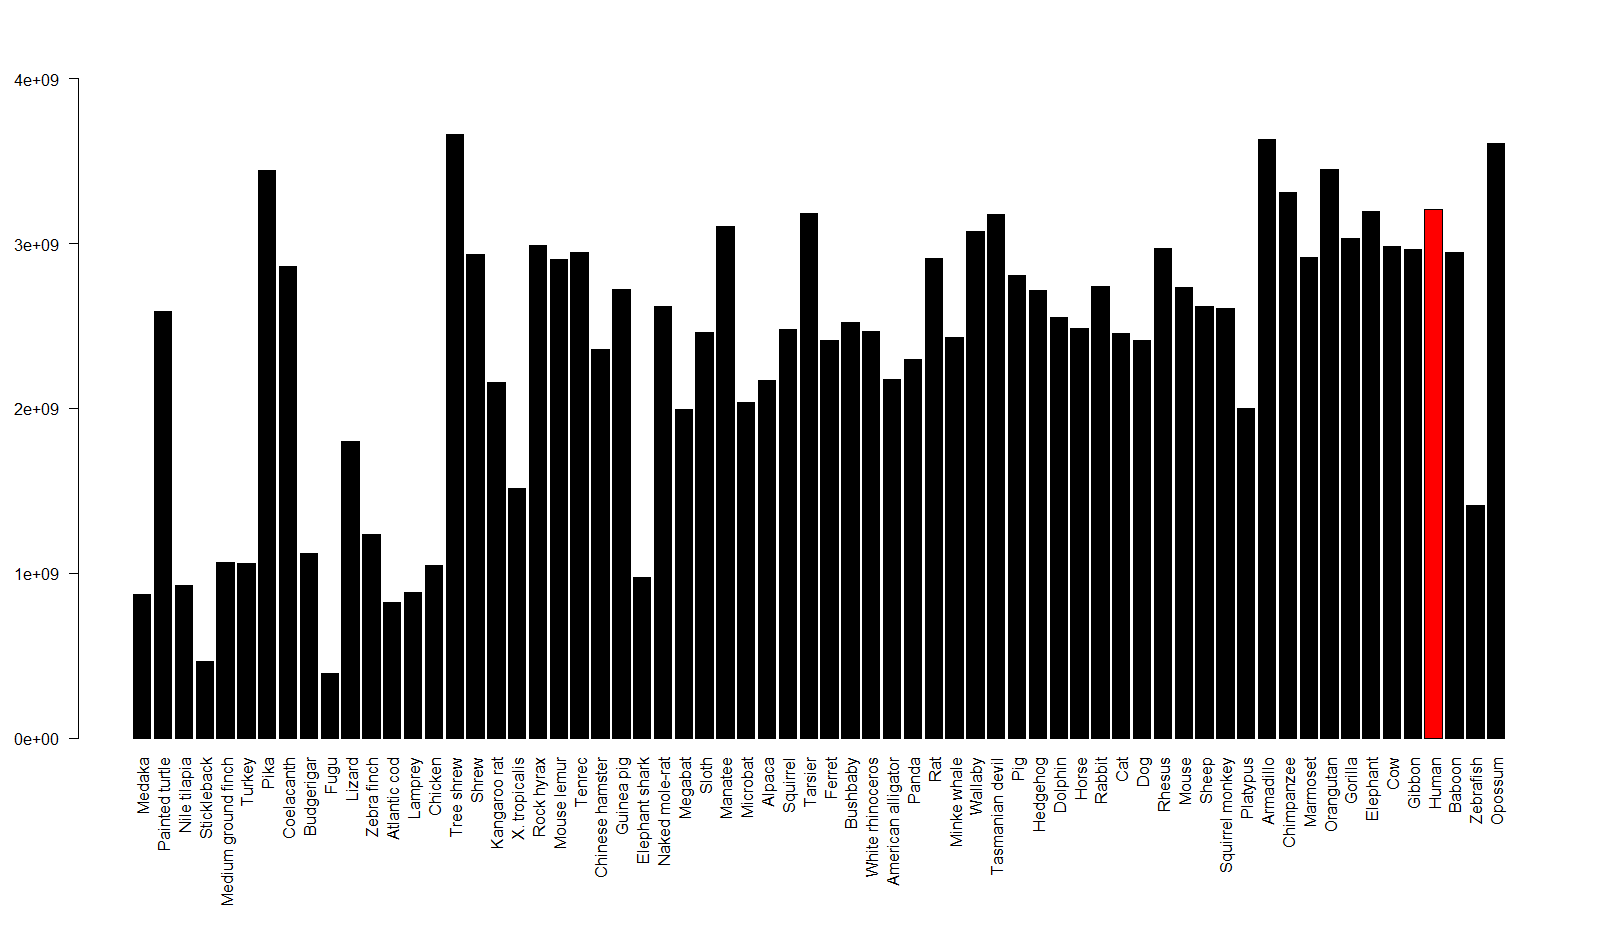
\includegraphics[width=\textwidth,natwidth=1600,natheight=932]{genome_size.png}
   \caption[Vertebrate genomes sizes]{The genome sizes of 66 vertebrate genomes, sorted from the lowest to highest percent of repetitive element coverage\cite{tang2014gensize}.}
   \label{fig:genome_size}
\end{figure}

\begin{figure}[h]
   \centering
   \includegraphics[width=9cm, angle=270]{barplot_repeat_family.eps}
   \caption[Tally of repetitive element families in the hg19 genome]{The number of repetitive element families determined by RepeatMasker in the hg19 genome.}
   \label{fig:repeat_family}
\end{figure}

\begin{itemize}
   \item Messenger RNAs are transcripts of protein-coding genes and are translated into protein
   \item Classical non-coding RNA found in both prokaryotes and eukaryotes are ribosomal RNAs and transfer RNAs, which are both involved in protein synthesis
   \item Diverse class of non-coding RNAs, broadly broken down into long and short non-coding RNA
   \item Assembly of non-coding RNAs with proteins as ribonucleoprotein (RNP) structures
   \item Interaction of non-coding RNAs with chromatin
   \item Pervasive transcription describes the observation that a large percentage of DNA in mammalian genomes is transcribed.
   \item Tiling arrays and full length cDNA sequencing suggested that most of the genome is transcribed
   \item The ENCODE pilot project provided multiple lines of evidence that most of the mammalian genome is associated with at least one primary transcript, i.e., pervasive transcription of the genome
   \item Are the majority of detected low-level transcription due to technical artifacts and/or background biological noise?
   \item Protocols that capture only poly-A transcripts as opposed to poly-A minus and cytoplasmic versus nuclear enrichment libraries
   \item Sequencing depth and sampling of RNA molecules; absolute transcript quantification will help (such as using unique molecule identifiers and non-PCR based methods)
   \item Functional transcriptomics in the post-ENCODE era, specifically what is the criteria for functionality
   \item Repeat-associated binding sites (RABS) are over-represented in proximity of regulated genes and that the binding motifs within these repeats have undergone evolutionary selection
   \item Indeed, studies conducted both at the gene and genome levels have uncovered TE insertions that seem to have been co-opted - or exapted - by providing transcription factor binding sites (TFBSs) that serve as promoters and enhancers, leading to the hypothesis that TE exaptation is a major factor in the evolution of gene regulation.
   \item The transcription of repetitive elements, especially transposable elements, in specific tissues
   \item Repetitive elements are usually highly methylated, however differentiation methylation patterns of repetitive elements was observed in specific tissues
   \item Functions of some GWAS candidates in intergenic regions (such as http://www.nature.com/nature/journal/v507/n7492/full/nature13138.html)
\end{itemize}

\section{Stem cells}

\begin{itemize}
   \item Stem cells have two key characteristics that make them different from other cells
   \item They can reproduce themselves for long periods of time; this is known as self-renewal and
   \item They can differentiate or specialise into specific cell types under certain conditions
   \item Embryonic stem cells are derived from the inner cell mass of blastocysts. In normal development, the inner cell mass begins growing into all the different cell types of the fully developed body
   \item In our fully developed bodies, we have some self-renewing cells that reside in a specific tissue that are able to generate specific types of differentiated cells, i.e., they have limited differentiation ability. They were named adult stem cells because they reside in fully formed tissues.
   \item However, some adult stem cells have a transdifferentiation ability, which is that they can generate cells outside their own tissue type.
   \item They are also known as somatic stem cells or tissue stem cells.
   \item Haematopoietic stem cells (HSCs), which are somatic stem cells, reside in the medulla of the bone (bone marrow) and have the unique ability to give rise to all of the different mature blood cell types and tissues.
\end{itemize}
